\section{Effective Field Theory ReInterpretation}
\label{sec:EFT}
The unfolded cross-sections from data are reinterpreted to constrain the possible effects of new physics using a model-independent approach. The Effective Field Theory, along with the model and operators used, are briefly introduced in Section \ref{subsec:EFT_Intro}. Simulation of the EFT MC samples is discussed in Section \ref{subsec:EFT_EventGen}. The statistical fit to constrain the contributions from BSM physics, including statistical and systematic uncertainties, is discussed in Section \ref{subsec:EFT_Method}, and finally, Section \ref{subsec:EFT_Results} presents the obtained results. 

\subsection{Introduction}
\label{subsec:EFT_Intro}
Similar to the Fermi theory developed by Fermi to describe the beta decay before the formulation of the electroweak theory, the effects of BSM physics with any new heavy resonances and short range can be described with a model-independent EFT approach at low energy scales. Due to its large mass, the potential new resonance can affect processes below the cut-off scale $\Lambda$ only through a virtual propagator, thus modifying the cross-sections for low-energy physics processes. The Lagrangian, including the new physics beyond the cut-off scale $\Lambda$, can be written through a Standard Model Effective Field Theory (SMEFT) formalism, where new physics describing operators are built with higher dimensions in the energy of SM fields. The SM Langrangian is dimension four in energy, and the SMEFT Lagrangian conserving the $SU(3)_{C} \otimes SU(2)_{L} \otimes U(1)_{Y}$ symmetry is constructed by adding new interactions through the SM field operators with dimensions greater than four ($d>4$) as, 
\begin{equation}
\label{eqn:L_SMEFT}
\mathcal{L}_{SMEFT} = \mathcal{L}_{SM} + \sum_{d \geq 5}\sum_{i}\frac{c_{i}^{d}}{\Lambda^{d-4}}\mathcal{O}_{i}^{d}
\end{equation}
where $\mathcal{O}_{i}^{d}$ is the higher dimension operator describing new physics with dimensionless coupling constants $c_{i}^{d}$, also known as the Wilson coefficients \cite{SMEFT}. 

Any SMEFT Lagrangian given by Equation \ref{eqn:L_SMEFT} should reduce to the SM at low energy scales and is required to respect the unitarity bound such that the amplitude of any EFT process cannot grow too fast with a given energy scale. There are one dimension-five operator and $20$ dimension-seven operators that meet all requirements of SMEFT \cite{SMEFT}\cite{Dim7_EFT}. However, these operators violate the conservation of either baryon or lepton numbers, which to date are experimentally observed to be conserved. Moreover, higher dimensions EFT operators are suppressed by the larger order of magnitude of the large cut-off energy scale. Therefore, in practice, only dimension-six and dimension-eight operators are considered to affect the low-energy processes measured at the LHC.

The main results of the analysis are the unfolded differential cross-sections in electroweak-enhanced phase space. Thus, the EFT constrains the operators that affect the electroweak processes shown by the Feynman diagrams in Figure \ref{fig:ZZjjFeynmanDiag_EWk}. There is a total of $59$ dimension-six SMEFT operators, and $26$ of them affect the electroweak processes by modifying either the self-interactions of the gauge bosons, the Higgs-vector boson interactions, $Z \rightarrow \ell \ell$ vertices or the purely fermionic fields affecting either the four-leptons or lepton-quark interactions. However, based on an initial sensitivity study using SM predicted Asimov\footnote{SM predicted detector-level distributions where the bin errors are the Poissonian errors derived from the weighted event counts.} dataset, it was observed that the constraints on these operators were more competent in processes with more significant statistics such as inclusive four lepton measurements presented in Ref \cite{Inclusive_FourLepton} or a global SMEFT fit using LEP, ATLAS, and CMS data discussed in Ref \cite{GlobalEFT_Dim6}. Therefore, in this thesis, only dimension-8 operators affecting the electroweak $pp\rightarrow ZZ^* (\rightarrow 4 \ell) jj$ processes will be considered. 

The quartic vector boson self-interactions are experimentally accessible with the LHC Run-2 dataset for the first time. There are EFT operators that modify the QGC vertex shown in Figure \ref{fig:ZZjjFeynmanDiag_EWk_b}, resulting in anomalous Quartic Gauge Couplings (aQGC). The aQGC operators relevant to the measurement are defined by the Eboli Model discussed in detail in Ref \cite{EFT_Eboli}. Table \ref{tab:aQGC_Operators} shows the $18$ dimension-8 operators from the Eboli model that give aQGC for processes involving multi-boson final states either by modifying the SM electroweak interactions or by introducing the SM forbidden neutral couplings such as $ZZZZ$, $ZZZA$, $ZZAA$, $ZAAA$ and $AAAA$. Among these $18$ operators, eight shown in Table \ref{tab:Dim8Operators} formed by the combination of different field strength tensors only affects the quartic gauge-self interactions of the vector bosons scattering without any impact to the triple self-interactions or Higgs-mediated processes. The measurement constraints these eight \textit{genuine-QGC operators}. 

\begin{table}[h]
    \caption{Eighteen dimension-8 operators from the Eboli model giving anomalous quartic gauge vertices in several multi-boson processes.\label{tab:aQGC_Operators}}
    \begin{center}
    \begin{tabular}{c|ccccccccc}
        \hline 
        & {\scriptsize{}WWWW} & {\scriptsize{}WWZZ} & {\scriptsize{}ZZZZ} & {\scriptsize{}WWAZ} & {\scriptsize{}WWAA} & {\scriptsize{}ZZZA} & {\scriptsize{}ZZAA} & {\scriptsize{}ZAAA} & {\scriptsize{}AAAA}\tabularnewline
        \hline
        \hline 
        {\footnotesize{}$\mathcal{O}_{S,0}$,$\mathcal{O}_{S,1}$} & {\scriptsize{}x} & {\scriptsize{}x} & {\scriptsize{}x} &  &  &  &  &  & \tabularnewline
        {\footnotesize{}$\mathcal{O}_{M,0}$, $\mathcal{O}_{M,1}$, $\mathcal{O}_{M,6}$, $\mathcal{O}_{M,7}$} & {\scriptsize{}x} & {\scriptsize{}x} & {\scriptsize{}x} & {\scriptsize{}x} & {\scriptsize{}x} & {\scriptsize{}x} & {\scriptsize{}x} &  & \tabularnewline
        {\footnotesize{}$\mathcal{O}_{M,2}$, $\mathcal{O}_{M,3}$, $\mathcal{O}_{M,4}$, $\mathcal{O}_{M,5}$} &  & {\scriptsize{}x} & {\scriptsize{}x} & {\scriptsize{}x} & {\scriptsize{}x} & {\scriptsize{}x} & {\scriptsize{}x} &  & \tabularnewline
        {\footnotesize{}$\mathcal{O}_{T,0}$, $\mathcal{O}_{T,1}$, $\mathcal{O}_{T,2}$} & {\scriptsize{}x} & {\scriptsize{}x} & {\scriptsize{}x} & {\scriptsize{}x} & {\scriptsize{}x} & {\scriptsize{}x} & {\scriptsize{}x} & {\scriptsize{}x} & {\scriptsize{}x}\tabularnewline
        {\footnotesize{}$\mathcal{O}_{T,5}$, $\mathcal{O}_{T,6}$, $\mathcal{O}_{T,7}$} &  & {\scriptsize{}x} & {\scriptsize{}x} & {\scriptsize{}x} & {\scriptsize{}x} & {\scriptsize{}x} & {\scriptsize{}x} & {\scriptsize{}x} & {\scriptsize{}x}\tabularnewline
        {\footnotesize{}$\mathcal{O}_{T,8}$, $\mathcal{O}_{T,9}$} &  &  & {\scriptsize{}x} &  &  & {\scriptsize{}x} & {\scriptsize{}x} & {\scriptsize{}x} & {\scriptsize{}x}\tabularnewline
        \hline
    \end{tabular}
    \end{center}
\end{table}

\begin{table}[h]
    \caption{The eight genuine QGC dimension-8 operators constrained by the measurement. \label{tab:Dim8Operators}}
    \begin{center}
    \begin{tabular}{| c | c | c | }
        \hline 
        Operators & Definition & Wilson Coefficient \\
        \hline
         & & \\
        $\mathcal{O}_{T,0}$ & $Tr[ \hat{W_{\mu\nu}} \hat{W^{\mu\nu}}] \times Tr[\hat{W_{\alpha \beta}} \hat{W^{\alpha \beta}} ] $ & $f_{T0}$ \\
         & & \\
        $\mathcal{O}_{T,1}$ & $Tr[ \hat{W_{\alpha\nu}} W^{\mu\beta}] \times Tr[ \hat{ W_{\mu \beta}}\hat {W^{\alpha \nu}} ] $ & $f_{T1}$ \\
         & & \\
        $\mathcal{O}_{T,2}$ & $Tr[ \hat{W_{\alpha\mu}} \hat{W^{\mu\beta} }] \times Tr[\hat{W_{\beta\nu}} \hat{W^{\nu\alpha} }] $ & $f_{T2}$ \\
         & & \\
        $\mathcal{O}_{T,5}$ & $Tr[ \hat{W_{\mu\nu}} \hat{W^{\mu\nu} } ] \times B_{\alpha\beta}B^{\alpha\beta} $ & $f_{T5}$ \\
         & & \\
        $\mathcal{O}_{T,6}$ & $Tr[ \hat{W_{\alpha\nu}} \hat{W^{\mu\beta} } ] \times B_{\mu\beta}B^{\alpha\nu} $ & $f_{T6}$ \\
         & & \\
        $\mathcal{O}_{T,7}$ & $Tr[ \hat{W_{\alpha\mu}} \hat{W^{\mu\beta} }] \times  B_{\beta\nu}B^{\nu\alpha} $ & $f_{T7}$ \\
         & & \\
        $\mathcal{O}_{T,8}$ & $ B_{\mu\nu}B^{\mu\nu}B_{\alpha\beta}B^{\alpha\beta} $ & $f_{T8}$ \\
         & & \\
        $\mathcal{O}_{T,9}$ & $ B_{\alpha\mu}B^{\mu\beta} B_{\beta\nu}B^{\nu\alpha}$ & $f_{T9}$ \\
        \hline 
    \end{tabular}
    \end{center}
\end{table}    

The amplitude of a process, including the aQGC EFT operators, depends on the SMEFT matrix element $\mathcal{M}_{SMEFT}$ which can be written as, 
\begin{equation}
    \mathcal{M}_{SMEFT} = \mathcal{M}_{SM} + \sum_{i}{ \frac{c_{i}}{\Lambda^4}\mathcal{M}_{i}}
    \label{eqn:SMEFTMatrixElem}
\end{equation}
where $\mathcal{M}_{SM}$ is the SM matrix element and $\mathcal{M}_{i}$ is the matrix element of the EFT operator $\mathcal{O}_{i}$. Similarly, the cross-section depends on the square of the matrix element $\mathcal{M}_{SMEFT}$, which is 
\begin{equation}
    |\mathcal{M}_{SMEFT}|^2 = |\mathcal{M}_{SM}|^{2} + 2 \sum_{i}{ \frac{c_{i}}{\Lambda^4} \textit{Re}(\mathcal{M}_{SM}^{*} \mathcal{M}_{i}}) + \sum_{i,j}{ \frac{c_{i}c_{j}}{\Lambda^8} \textit{Re}(\mathcal{M}_{i}^{*} \mathcal{M}_{j}})
    \label{eqn:SMEFT_SQMatrixElem}
\end{equation}
In the measurement, only one EFT operator is constrained per fit. Therefore there is no need to consider the interference between the two EFT operators represented by the last term. Thus, simplifying Equation \ref{eqn:SMEFT_SQMatrixElem} to, 
\begin{equation}
    |\mathcal{M}_{SMEFT}|^2 = |\mathcal{M}_{SM}|^{2} + 2 \sum_{i}{ \frac{c_{i}}{\Lambda^4} \textit{Re}(\mathcal{M}_{SM}^{*} \mathcal{M}_{i}}) + \sum_{i,j}{ \frac{c_{i}^2}{\Lambda^8} |\mathcal{M}_{i}|}
    \label{eqn:SMEFT_CrossSec}
\end{equation}
where the second term is the \textit{linear-only EFT term} representing the interference in the matrix element between SM and EFT, and the last term is the \textit{quadratic term} representing the pure EFT-only contribution. The analysis uses a full EFT model considering effects from both the interference and the quadratic term. 

The SMEFT predicted cross-section for a single operator involving aQGC vertex is thus given as 
\begin{equation}
\sigma_{SMEFT}^{pred} = \sigma_{SM}[ 1 + c . A_{Int} + c^2 . B_{Quad} ]
\end{equation}
where $A_{Int}$ and $B_{Quad}$ are the corresponding relative linear and quadratic EFT contributions. The same is true when comparing the differential cross-sections, where cross-sections are compared in each bin. 

\subsection{Event Generation}
\label{subsec:EFT_EventGen}
The EFT samples are generated for each dimension-8 EFT operator using \textsc{MadGraph5} at leading order using the NNPDF3.0NLO PDF set and ignoring all the QCD vertices.
All Feynman diagrams contributing to the inclusive $pp \rightarrow ZZ^* jj$ process are first generated using \textsc{MadGraph5} and interfaced with \textsc{Pythia8} to simulate parton showering, hadronization, and multiparton interaction. Some generator-level kinematic selections such as $\eta_{j}<5$, $p_{T,j} > 15$ GeV, and $m_{jj} > 10$ GeV are applied to speed up the generation process. Each $Z$-boson is then decayed leptonically ($Z\rightarrow \ell \ell$) using \textsc{MadSpin}. For each EFT operator, the cross-sections for linear-only and quadratic-only terms are generated by setting the value of the relevant Wilson coefficient to $1$ and the value of all other Wilson coefficients to $0$. The differential cross-section in bin $i$ for any value of the Wilson coefficient is then estimated by utilizing the following relation,
\begin{equation}
\frac{d\sigma ^{i}}{dX}(c) = \frac{d\sigma ^{i}_{SM}}{X} + c . \frac{d\sigma ^{i}_{Int, c=1}}{dX} + c^2 . \frac{d\sigma ^{i}_{Quad, c=1}}{dX}
\label{eqn:DiffxS_EFT}
\end{equation}

\subsection{Statistical Strategy for Limit Setting}
\label{subsec:EFT_Method}
A profile likelihood technique \cite{ProfileLikelihood} is used to constrain each Wilson coefficient at $95\%$ confidence level. The method relies on building a chi-square ($\chi^2$) statistic that measures the compatibility between the differential cross-sections predicted by SMEFT ($\vec{\sigma}_{pred}$) to the unfolded differential cross-sections either from the predicted Asimov data or measured data ($\vec{\sigma}_{data}$). For a given value of a selected Wilson Coefficient $c_X$, the $\chi^2$ is given by
\begin{equation}
    \chi^2(c_X, \vec{\theta}) = [\vec{\sigma}_{data} - \vec{\sigma}_{pred}(c_X)- \sum_{\theta}\theta\cdot\vec{e_\theta} ]^T \textbf{C}^{-1}[\vec{\sigma}_{data}  - \vec{\sigma}_{pred}(c_X) - \sum_{\theta}\theta\cdot\vec{e_\theta}],
    \label{eq:eftchi2}
\end{equation} 
where $\textbf{C}$ is the total statistical and systematic covariance matrices on measured differential cross-sections ($\vec{\sigma}_{data}$) and $\theta$ is a vector including all nuisance parameters, where each component corresponds to a particle-level uncertainty on SM prediction with an absolute magnitude of $e_{\theta}$.

The likelihood function gives a conditional probability, encoding the probability of observing the data under the assumption of the SMEFT model, and is constructed as 
\begin{equation}
    \mathcal{L}(c_X, \vec{\theta}) = \frac{1}{\sqrt{(2\pi)^k\cdot|\textbf{C}|}} \cdot e^{-\frac{1}{2}\chi^2(c_X, \vec{\theta})} \cdot \prod_{\theta}\mathcal{G}(\theta)
    \label{eqn:Likelihood}
\end{equation}
where $k$ is the number of measurements equal to the length of $\vec{\sigma}_{data}$. $\mathcal{G}(\theta)$ is the Gaussian-constrained nuisance parameter $\theta$ with a mean of zero and standard deviation of one. 

The profile likelihood ratio test statistic for a SMEFT model depending on a single parameter $c$ is defined as
\begin{equation}
    q(c) = -2 \ln \frac{\mathcal{L}(c, \hat{\hat{\vec{\theta}}}(c))}{\mathcal{L}(\hat{c}, \hat{\vec{\theta}}(c))}
\label{eq:teststat}
\end{equation}
where $\hat{c}$ and $\hat{\vec{\theta}}(c)$ in the denominator are the unconditional maximum likelihood estimators of $c$ and $\vec{\theta}(c)$, while $\hat{\hat{\vec{\theta}}}(c)$ is the value of $\vec{\theta}$ which maximizes the likelihood for a given value of $c$. Following the definition of the test statistic in Equation \ref{eq:teststat}, likelihood in Equation \ref{eqn:Likelihood} and $\chi^2$ in Equation \ref{eq:eftchi2} and implementing the logarithmic relations, the test statistics simplifies to a summation of two terms: the $\Delta \chi^2$ and difference in the sum of quadrature over the nuisance parameters as, 
\begin{equation}
    q(c) = \Delta \chi^2 + \Delta \sum_{i}{\Theta^2}
    \label{eqn:SimplifiedTestStat}
\end{equation}
Low test statistic values closer to zero infer a good agreement between the measured unfolded cross-sections and the SMEFT-predicted cross-sections. According to Wilk's theorem, the test statistic distribution in Equation \ref{eq:teststat} asymptotically approaches the $\chi^2$ distribution for one degree of freedom \cite{WilksTheorem}. Therefore, the $95\%$ confidence limits (CL) for a Wilson coefficient are constructed assuming Wilk's theorem by excluding values of $c$ for which
\begin{equation}
    \int_{0}^{q(c)} \chi^2(d.o.f = 1) \, dq > 95 \%,
\label{eq:chi2cdf}
\end{equation}
In $95\%$ C.L. and one degree of freedom, the upper limit of the q-value should be 3.84. 

In the measurement, a one-dimensional unfolded differential cross-section distribution of $m_{jj}$ appended to the last four bins of $m_{4\ell}$ distribution is used to constrain the dimension-8 Eboli EFT operators. This choice of combined $1D$ observable is motivated to maximize the sensitivity by using two observables but the inability to construct a full $2D$ observable due to low statistics. Both $m_{jj}$ and $m_{4\ell}$ distributions describe the same event, and using a full combined distribution overconstrains the limits obtained from the fit. Therefore, the first bin of $m_{4\ell}$ with no sensitivity to the EFT contribution is removed. \\
\textbf{Covariance of the Unfolded Cross-sections (C)}\\
The covariance used in Equations \ref{eq:eftchi2} and \ref{eqn:Likelihood} is a total sum of the statistical covariance matrix shown in Figure \ref{fig:StatCov_mjj_m4l} and the systematic covariance matrix shown in Figure \ref{fig:SysCov_mjj_m4l}. The statistical covariance is estimated by the \textit{Bootstrapping method} discussed in detail in Ref \cite{Bootstrapping}, which generates a pseudo-detector-level dataset following a Poisson distribution with a mean one. Ten thousand toy replicas are generated by varying the content of each bin and unfolded using unfolding inputs from the nominal SM prediction. The correlation between the unfolded replica-distributions gives the covariance shown in Figure \ref{fig:StatCov_mjj_m4l}.

The systematic covariance matrix includes all sources of theoretical, experimental, and unfolding uncertainties discussed in Section \ref{sec:Uncertainties}. The covariance is constructed by assuming each systematic uncertainty to be $100\%$ correlated between bins and uncorrelated from any other systematic uncertainty. For instance, if the $n^{th}$ systematic uncertainty of the $i^{th}$ bin is the difference between the nominal and variation-applied yield $\delta_{n, i}$, then the systematic covariance in bin $ij$ is given by summing the product of the difference over all various sources of uncertainties,
\begin{equation}
C^{syst.}_{ij} = \sum_{n}\delta_{n, i}\delta_{n, j}
\end{equation} 

\begin{figure}[!htb]
    \centering
    \begin{subfigure}{.49\textwidth}
        \centering
        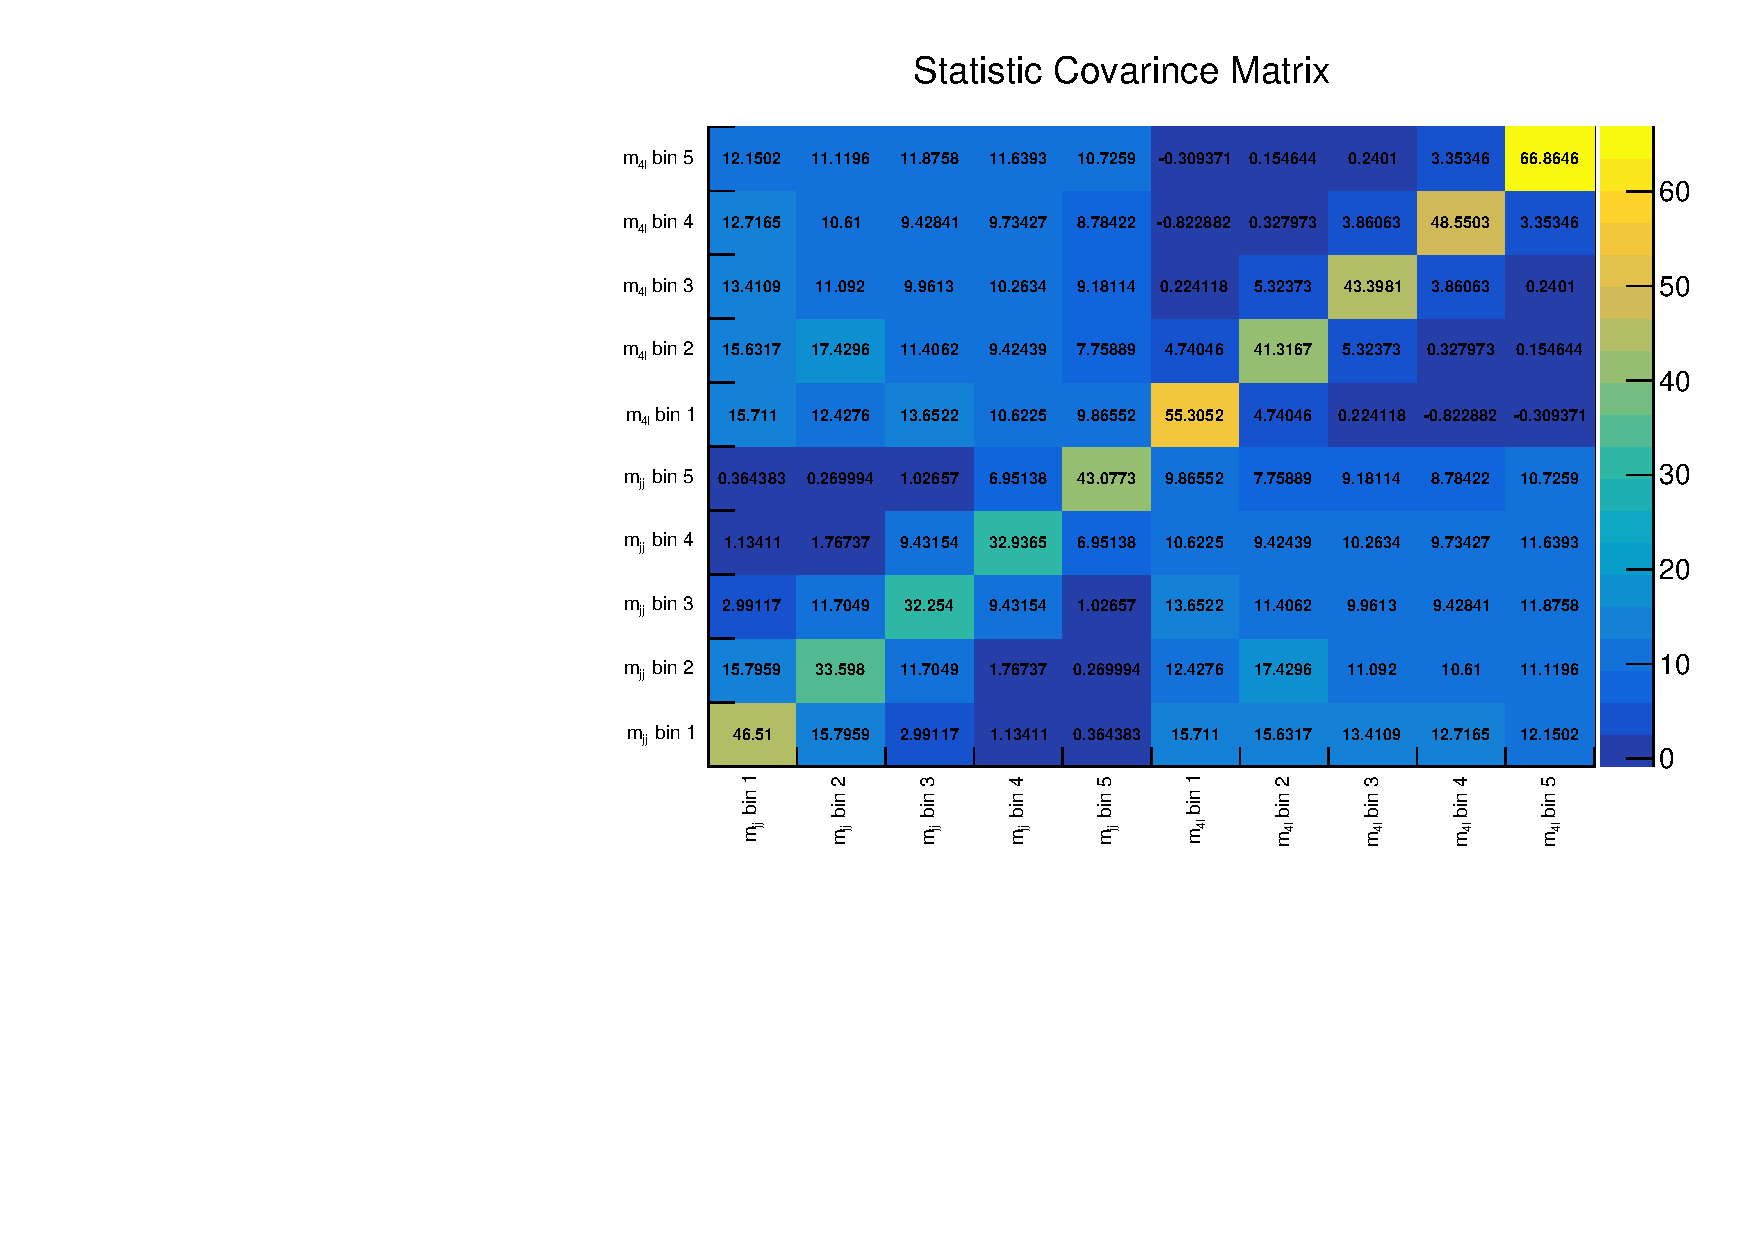
\includegraphics[width=.98\linewidth]{figures/Results/EFT/Cov_stat.pdf}
        \caption{ Statistics Covariance Matrix \label{fig:StatCov_mjj_m4l}}
    \end{subfigure}
    \begin{subfigure}{.49\textwidth}
        \centering
        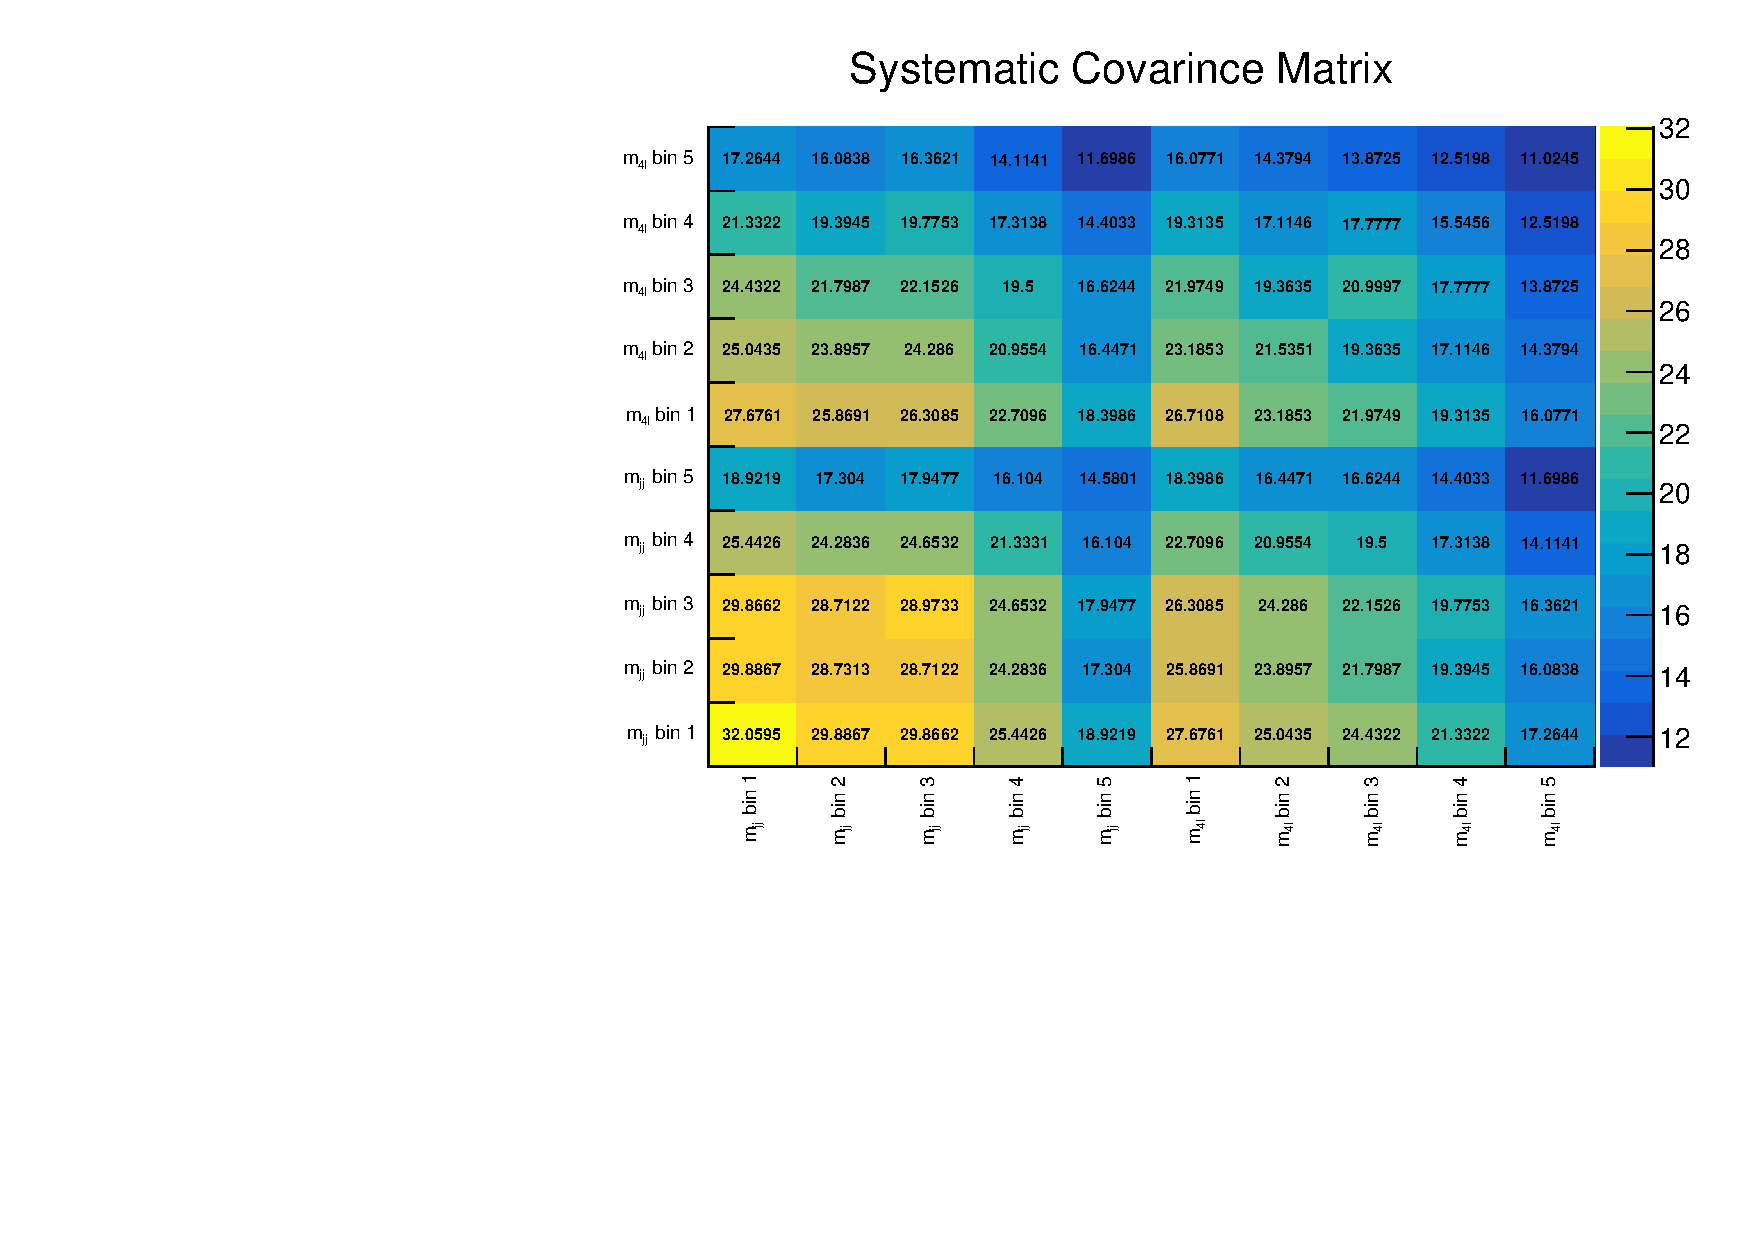
\includegraphics[width=.98\linewidth]{figures/Results/EFT/Cov_syst.pdf}
        \caption{ Systematics Covariance Matrix \label{fig:SysCov_mjj_m4l} }
    \end{subfigure}
    \caption{Covariance matrix for $m_{jj}+m_{4\ell}$ unfolded differential cross-sections in the VBS-Enhanced region. }  \label{fig:Cov_mjj_m4l}
\end{figure}
\textbf{Nuissance Paremeters ($\theta$)} \\
The following particle-level uncertainties are considered as nuisance parameters in the profile likelihood fit,
\begin{itemize}
    \item{\textbf{QCD Scale}: The same scale variations discussed in Section \ref{subsec:TheoryUnc} are considered for the parton-initiated QCD $qqZZ$, gluon-loop initiated QCD $ggZZ$ and EWK $qqZZjj$ samples.} 
    \item{\textbf{QCD PDF $\& ~ \alpha_{S}$}: The same set of PDF and $\alpha_{S}$ at variations discussed in Section \ref{subsec:TheoryUnc} are considered at the particle-level for the parton-initiated QCD $qqZZ$, gluon-loop initiated QCD $ggZZ$ and EWK $qqZZjj$ samples. }
    \item{\textbf{ggZZ NLO Reweighting}: Uncertainty on the k-factor for the $ggZZ$ sample is also taken into account. }
    \item{\textbf{QCD Modeling Uncertainties}: This uncertainty accounts for the modeling differences in the QCD $qqZZ$ samples and is estimated by taking the difference between \textsc{Sherpa} and \textsc{MadGraph} predictions.} 
\end{itemize}

Figure \ref{fig:EFT_Example} shows an example of setting constraints on one dimension-8 $\mathcal{O}_{T,0}$ operator with the cut-off energy scale set to $1$ TeV. The example uses the unfolded cross-sections from the Asimov dataset. Figure \ref{fig:EFT_Example_LikelihoodScan} shows the likelihood scan as a function of different values of $f_{T0}$ Wilson coefficient for two cases; first, only including the statistical covariances, and second, including both statistical and systematic covariances for the unfolded cross-sections. The two respective curves represent different test statistic ($q$) values for different values of the Wilson coefficient. The intersection between the curves and the upper value of $q=3.84$ gives the $95\%$ confidence limit for the $f_{T0}$ Wilson coefficient to be $[-0.898,0.847]$. Figure \ref{fig:EFT_Example_MaxValue} shows the three distributions; SM predicted truth-level yield with fiducial-level theoretical uncertainties, the SMEFT truth-level prediction when the value of $f_{T0}$ Wilson coefficient equals $0.847$, the upper limit from the fit, as well as the unfolded SM Asimov data with statistical, experimental, theoretical, and unfolding uncertainties. Enhancements of about $20-25\%$ on the last bin of $m_{jj}$ and $m_{4\ell}$ are observed when the EFT contribution is maximum allowed by the expected upper limit value for $f_{T0}$. Similarly, Figures \ref{fig:EFT_Example_LikelihoodScan_Data} and \ref{fig:EFT_Example_MaxValue_Data} show the same but when using the unfolded cross-sections measured from data. 

\begin{figure}[!htb]
    \centering
    \begin{subfigure}{.49\textwidth}
        \centering
        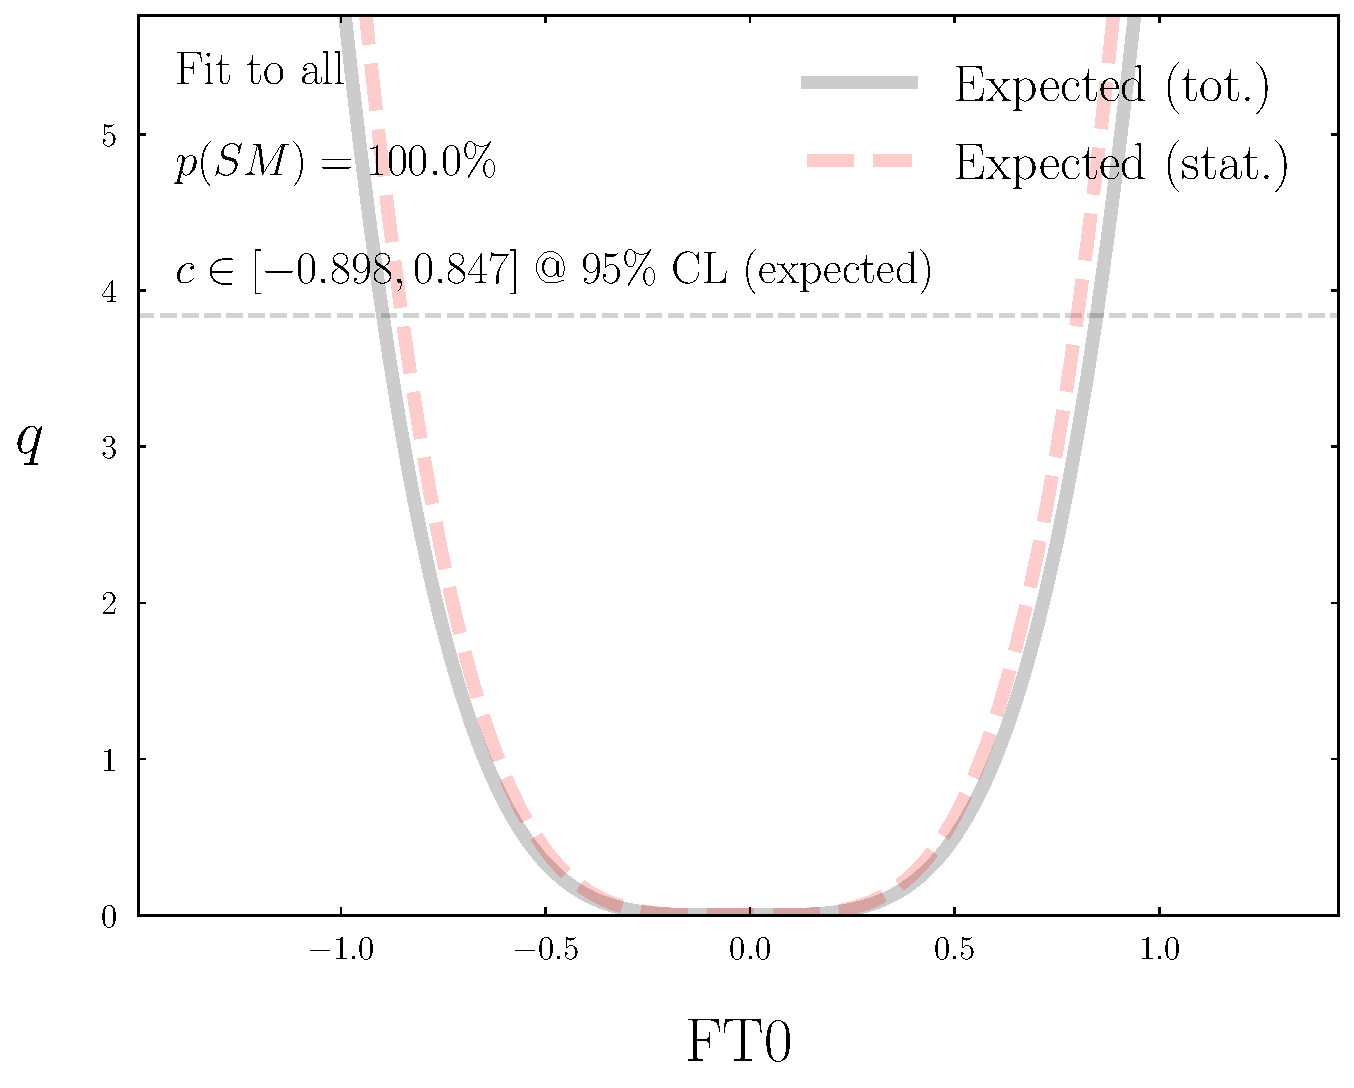
\includegraphics[width=.8\linewidth]{figures/Results/EFT/Likelihood_profile_FT0_all_SR_SM_fixed.pdf}
        \caption{ Likelihood scan \label{fig:EFT_Example_LikelihoodScan}}
    \end{subfigure}
    \begin{subfigure}{.49\textwidth}
        \centering
        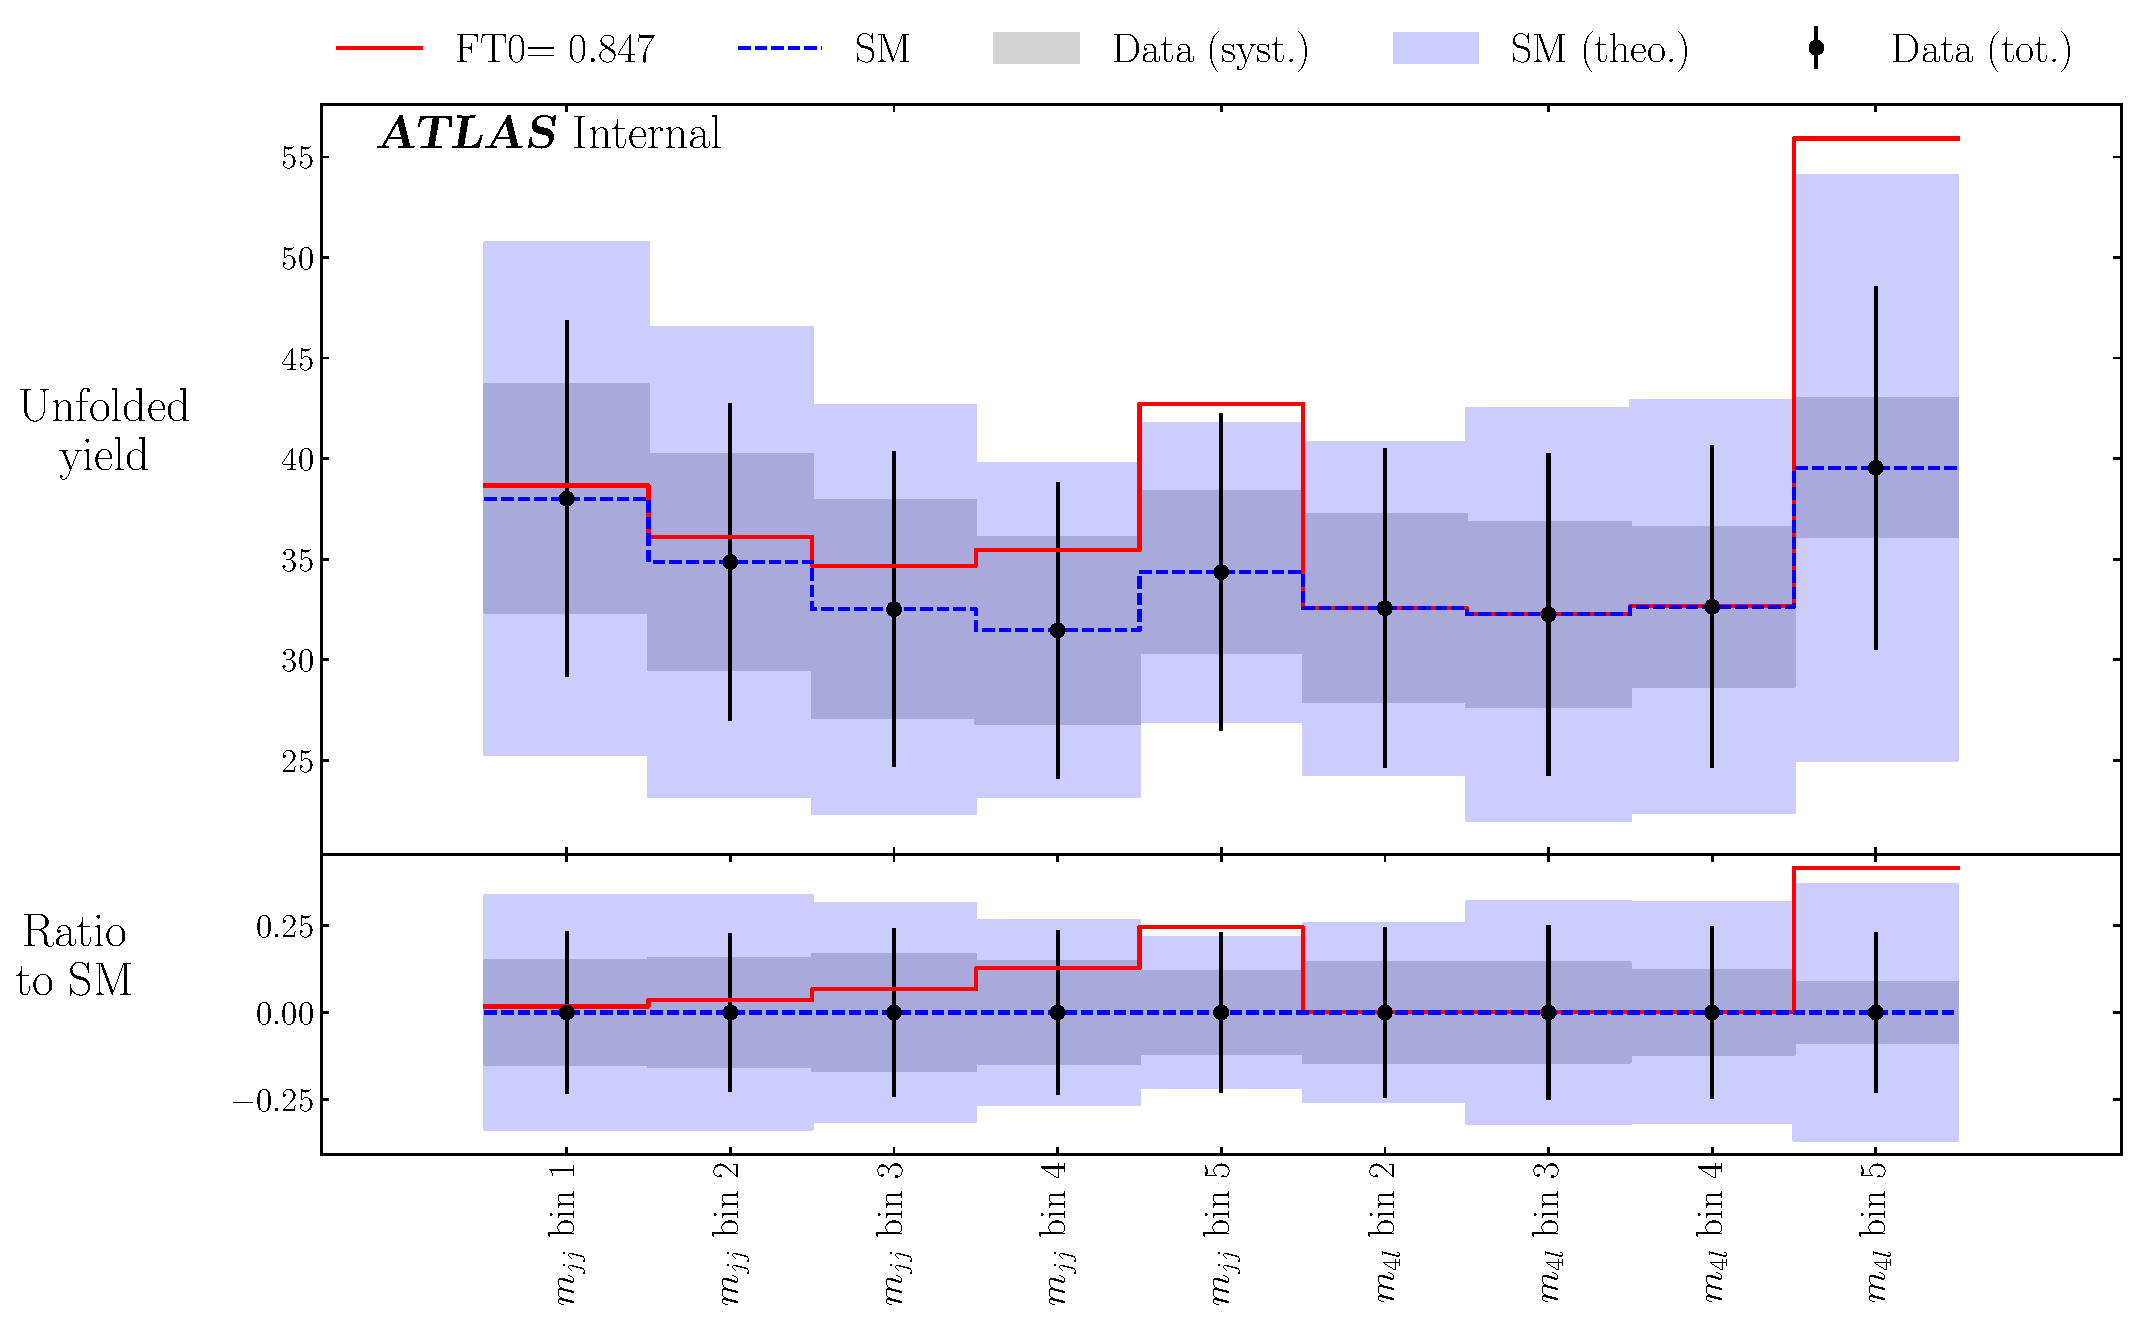
\includegraphics[width=.99\linewidth]{figures/Results/EFT/Unfolded_spectrum_FT0_all_SR_SM_fixed.pdf}
        \caption{ Unfolded-Asimov data and truth-level SM and EFT predictions.\label{fig:EFT_Example_MaxValue} }
    \end{subfigure}
    \caption{ An example of setting constraints on dimension-8 $\mathcal{O}_{T,0}$ EFT operator with one-dimensional $m_{jj}+m_{4\ell}$ Asmiov-unfolded differential cross-sections.  \label{fig:EFT_Example}}
\end{figure}

\begin{figure}[!htb]
    \centering
    \begin{subfigure}{.49\textwidth}
        \centering
        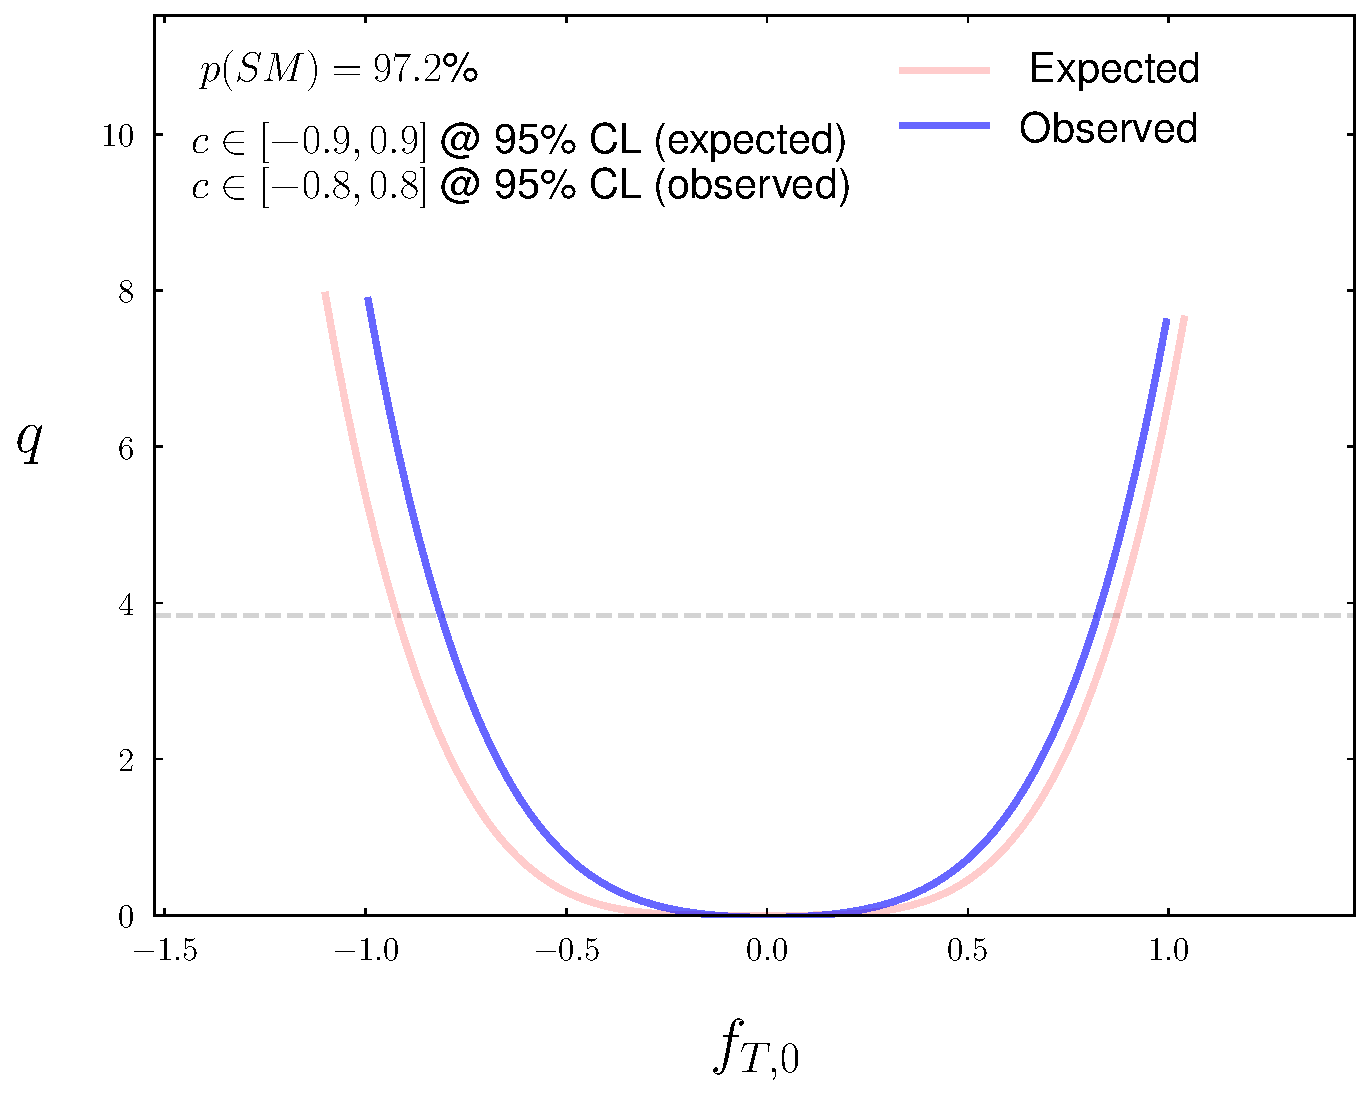
\includegraphics[width=.8\linewidth]{figures/Results/EFT/Likelihood_profile_FT0_mjj_m4l_SM_fixed_twoobs.pdf}
        \caption{ Likelihood scan \label{fig:EFT_Example_LikelihoodScan_Data}}
    \end{subfigure}
    \begin{subfigure}{.49\textwidth}
        \centering
        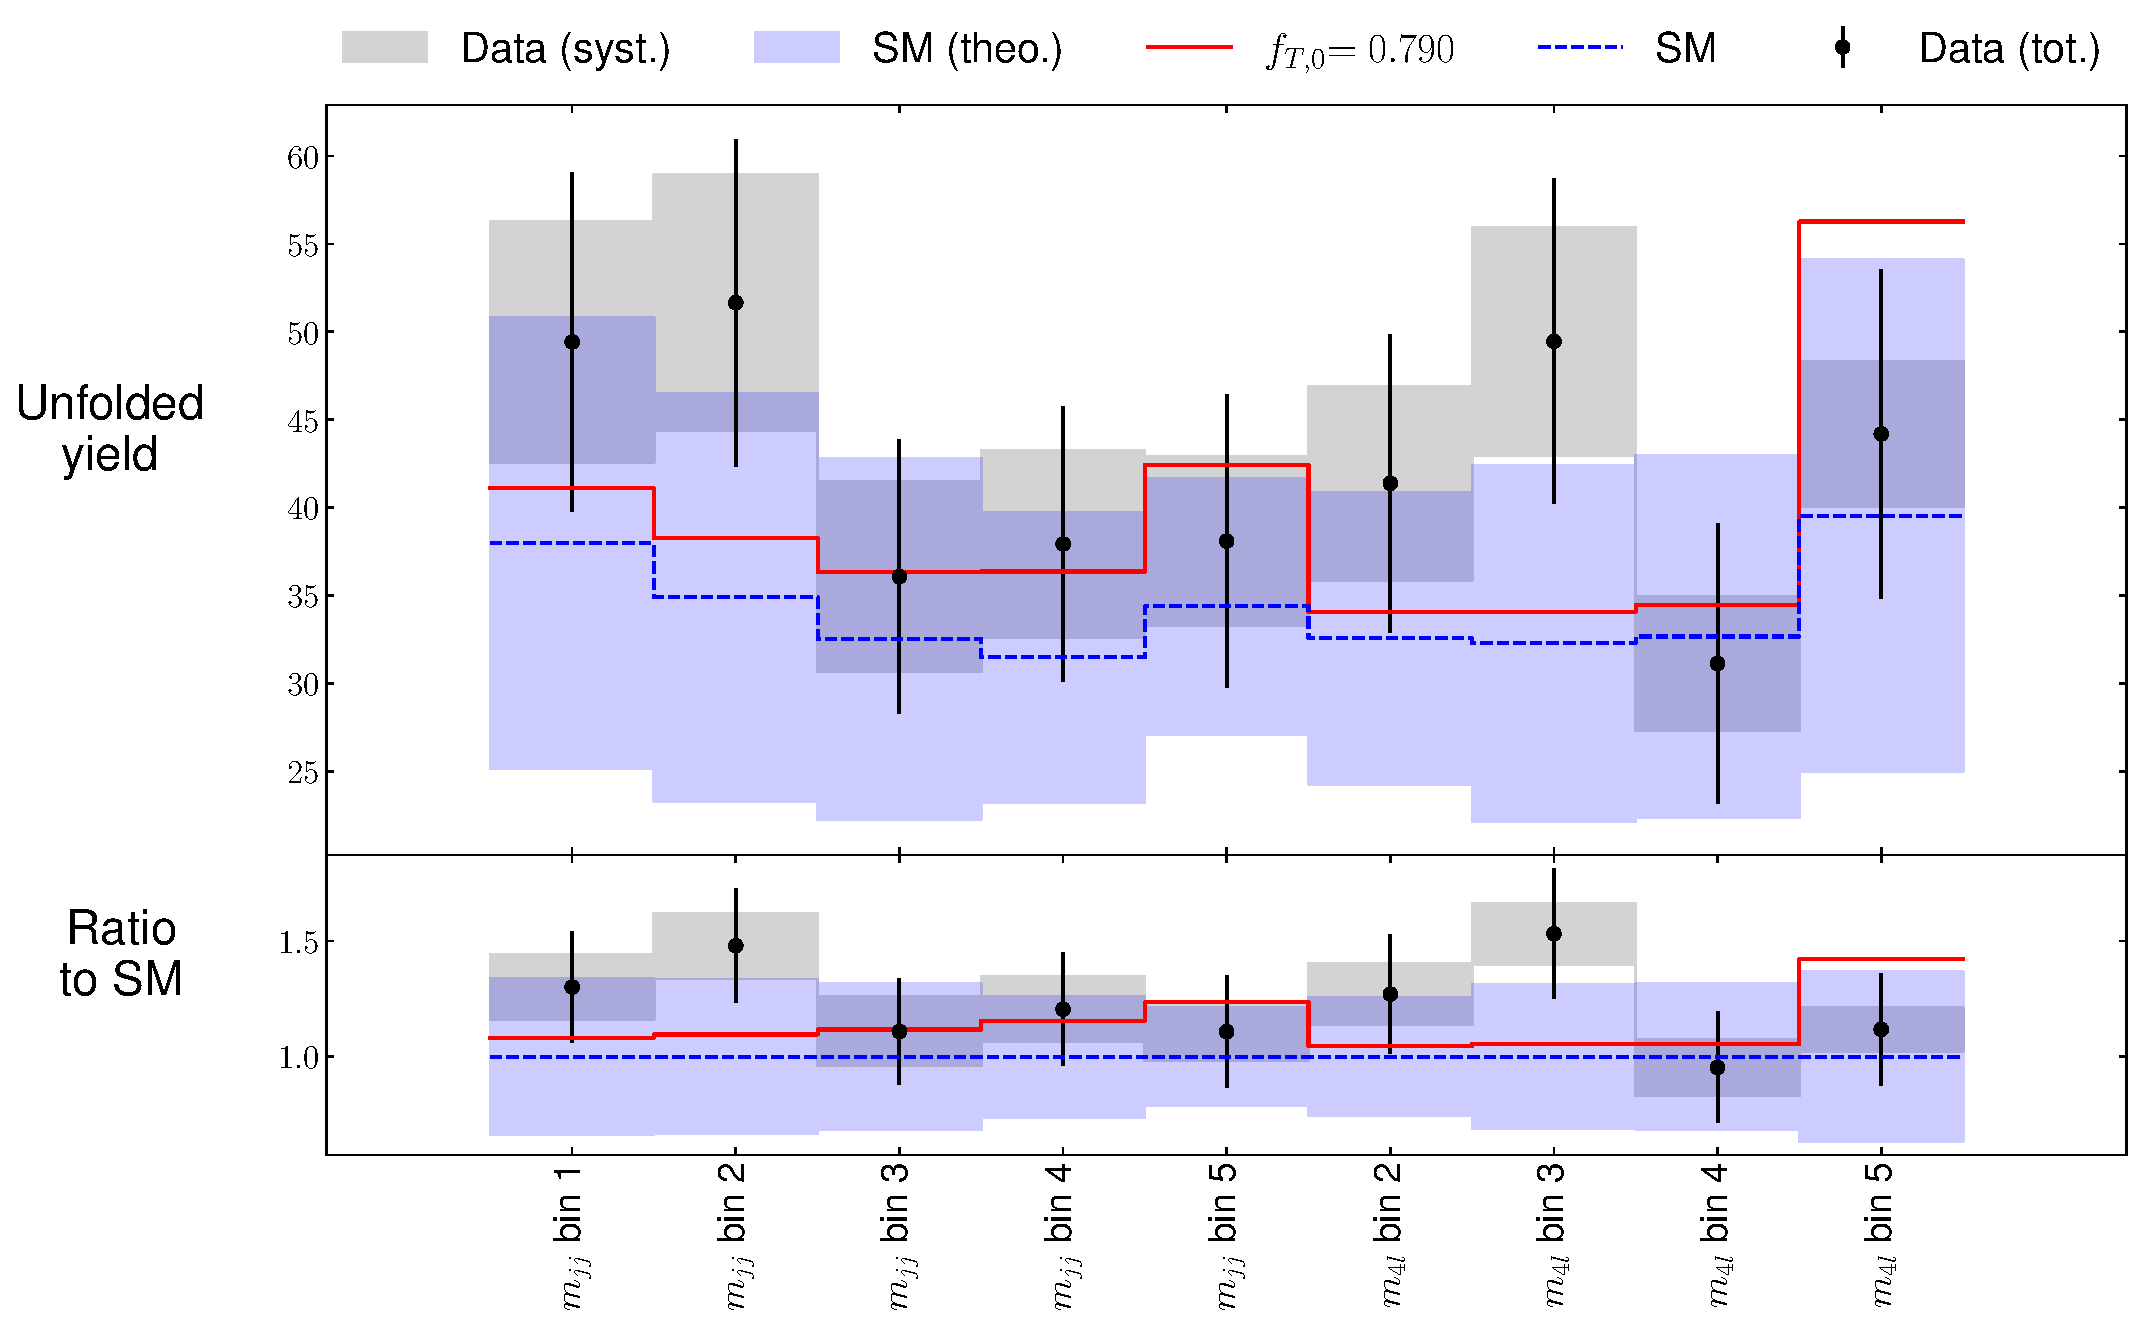
\includegraphics[width=.99\linewidth]{figures/Results/EFT/Unfolded_spectrum_FT0_mjj_m4l_SM_fixed_twoobs.pdf}
        \caption{ Unfolded data and truth-level SM and EFT predictions.\label{fig:EFT_Example_MaxValue_Data} }
    \end{subfigure}
    \caption{ An example of setting constraints on dimension-8 $\mathcal{O}_{T,0}$ EFT operator with one-dimensional $m_{jj}+m_{4\ell}$ unfolded differential cross-sections measured from data.  \label{fig:EFT_Example_Data}}
\end{figure}

\subsection{Results}
\label{subsec:EFT_Results}
The expected and observed $95\%$ confidence limits on the Wilson coefficients associated with the $8$ genuine QGC operators are shown in Table \ref{tab:twoobsofeboli}. The limits are obtained by fitting the unfolded differential cross-sections obtained from SM prediction and measured data, respectively. The competent observed limits are compatible with the expected limits using the SM predicted cross-sections. Therefore, it is concluded that the effects of new physics are not observed in the reinterpreted LHC Run-2 dataset.

\begin{table}[ht]
    \centering
    \caption{Expected and observed limits based on the unfolded Asimov and measured data, respectively, for the selected dimension-8 Wilson coefficients in Eboli Model. The limits are obtained by simultaneously fitting unfolded differential cross-sections of the $\mjj$ and $\mFourL$, including the overflow contribution in the VBS-Enhanced region. \label{tab:twoobsofeboli}}
    \begin{tabular}{| c | c | c |}
        \hline
        Wilson Coefficient &    Expected [Asimov]  & Observed [Data]         \\
        \hline\hline
        $f_{T0}$ &  $[-9.0, 8.5]\times 10^{-1}$  & $[-8.4, 7.9] \times 10^{-1}$ \\
        $f_{T1}$ &  $[-1.1, 1.1]$ & $[-1.0, 1.0]$ \\
        $f_{T2}$ &  $[-2.3, 2.2]$ & $[-2.2, 2.1]$ \\
        $f_{T5}$ &  $[-2.3, 2.2]$ & $[-2.2, 2.1]$ \\
        $f_{T6}$ &  $[-3.6, 3.6]$ & $[-3.3, 3.3]$ \\
        $f_{T7}$ &  $[-7.7, 7.4]$ & $[-7.2, 6.9]$ \\
        $f_{T8}$ &  $[-1.9, 1.9]$ & $[-1.8, 1.8]$ \\
        $f_{T9}$ &  $[-4.1, 4.1]$ & $[-3.9, 3.9] $\\                               
        \hline
    \end{tabular}
\end{table}